% -*- mode: latex; -*- mustache tags:  
\documentclass[10pt,twoside,english]{_support/latex/sbabook/sbabook}
\let\wholebook=\relax

\usepackage{import}
\subimport{_support/latex/}{common.tex}

%=================================================================
% Debug packages for page layout and overfull lines
% Remove the showtrims document option before printing
\ifshowtrims
  \usepackage{showframe}
  \usepackage[color=magenta,width=5mm]{_support/latex/overcolored}
\fi


% =================================================================
\title{A PharoThings Tutorial}
\author{Allex Oliveira}
\series{Square Bracket tutorials}

\hypersetup{
  pdftitle = {A PharoThings Tutorial},
  pdfauthor = {Allex Oliveira},
  pdfkeywords = {IoT, Raspberry, PharoThings, Pharo}
}


% =================================================================
\begin{document}

% Title page and colophon on verso
\maketitle
\pagestyle{titlingpage}
\thispagestyle{titlingpage} % \pagestyle does not work on the first one…

\cleartoverso
{\small

  Copyright 2017 by Allex Oliveira.

  The contents of this book are protected under the Creative Commons
  Attribution-ShareAlike 3.0 Unported license.

  You are \textbf{free}:
  \begin{itemize}
  \item to \textbf{Share}: to copy, distribute and transmit the work,
  \item to \textbf{Remix}: to adapt the work,
  \end{itemize}

  Under the following conditions:
  \begin{description}
  \item[Attribution.] You must attribute the work in the manner specified by the
    author or licensor (but not in any way that suggests that they endorse you
    or your use of the work).
  \item[Share Alike.] If you alter, transform, or build upon this work, you may
    distribute the resulting work only under the same, similar or a compatible
    license.
  \end{description}

  For any reuse or distribution, you must make clear to others the
  license terms of this work. The best way to do this is with a link to
  this web page: \\
  \url{http://creativecommons.org/licenses/by-sa/3.0/}

  Any of the above conditions can be waived if you get permission from
  the copyright holder. Nothing in this license impairs or restricts the
  author's moral rights.

  \begin{center}
    
\includegraphics[width=0.2\textwidth]{_support/latex/sbabook/CreativeCommons-BY-SA.pdf}
  \end{center}

  Your fair dealing and other rights are in no way affected by the
  above. This is a human-readable summary of the Legal Code (the full
  license): \\
  \url{http://creativecommons.org/licenses/by-sa/3.0/legalcode}

  \vfill

  % Publication info would go here (publisher, ISBN, cover design…)
  Layout and typography based on the \textcode{sbabook} \LaTeX{} class by Damien
  Pollet.
}


\frontmatter
\pagestyle{plain}

\tableofcontents*
\clearpage\listoffigures

\mainmatter

\chapter{Lesson 11 - Building a Mini-Weather Station}
In the previous lessons, we learned how to control LEDs, sensors, LCD displays and how to use OOP to create applications to control them. Now we will use everything that we learned to build a Mini-Weather Station. 
\section{What do we need?}
In this lesson, we will use a setup with an LCD Display 1602 and BME280 sensor.
\subsection{Components}
\begin{itemize}
\item 1 Raspberry Pi connected to your network (wired or wireless)
\item 1 Breadboard
\item 1 BME280 temperature, humidity and pressure sensor
\item 1 LCD Display 1602 
\item 1 Potentiometer (10K ohms)
\item Jumper wires
\end{itemize}
\section{Experimental theory}
Before constructing any circuit, you must know the parameters of the components in the circuit, such as their operating voltage, operating circuit, etc.

In this lesson, we will get the temperature, pressure, and humidity using the BME280 sensor, show this information on the LCD Display each 1 second and send this data to a Cloud Server every 60 seconds. 
\section{Experimental procedure}
Connect the sensor and LCD Display on your breadboard as we did in the previous lessons. 
\section{Creating the ThingSpeak account }
In order to store the measure collected by the weather station, we will use a web service called ThingSpeak. ThingSpeak is a cloud application that is dedicated to IoT (Internet of Things).

Before we start to create an application, let's create our account on the website Thingspeak. We will go to use this website to receive and store the data.

Follow this tutorial to create your account and your channel:

\textcode{https://roboindia.com/tutorials/thingspeak-setup}

Once you've created your channel, you need to enable three channels on it. Let's use Field1 to Temperature, Field2 to Humidity and Field3 to Pressure. You can see in Picture \ref{ThingspeakChannelConf} how your channel will look like.


\begin{figure}

\begin{center}
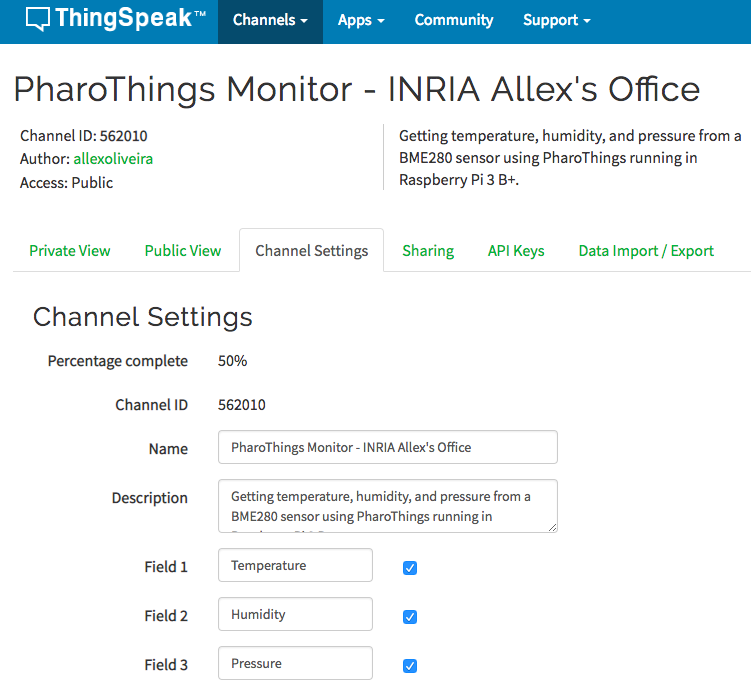
\includegraphics[width=0.85\textwidth]{/Users/allexoliveira/PharoThingsBook/Booklet-APharoThingTutorial/_result/pdf/Chapters/Chap12BuildingaMiniWeatherStation/figures/pharothings-thingspeak-conf.png}\caption{ThingSpeak Channel Configuration.\label{ThingspeakChannelConf}}\end{center}
\end{figure}


You can test your channel by simulating sending some data to it. Let's for example send the values:

\begin{itemize}
\item 25 to Temperature field (field1);
\item 56 to Humidity field (field2);
\item and 1012 to Pressure field (field3).
\end{itemize}

To test your channel, just copy the following URI and passed in your web browser, changing YOUR-WRITE-API-KEY to your ThingSpeak write API code. You can find it in the API Keys tab. 

\textcode{https://api.thingspeak.com/update?api\_key=YOUR-WRITE-API-KEY\&
field1=25\&field2=56\&field3=1012}

So check you channel to see if it was updated with this values:

\textcode{https://thingspeak.com/channels/YOUR-CHANNEL-ID}
\section{Creating the application}
The first step lets create a Superclass to initialize and install all devices that we will use. So let's create 2 subclasses to do the actions. The first will display this information on the LCD and the second will send the data to the cloud. Your final code will seem like the Picture \ref{MiniWeatherStationcode}.


\begin{figure}

\begin{center}
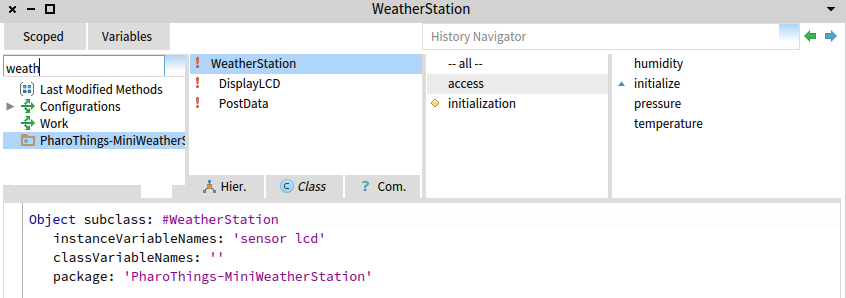
\includegraphics[width=0.85\textwidth]{/Users/allexoliveira/PharoThingsBook/Booklet-APharoThingTutorial/_result/pdf/Chapters/Chap12BuildingaMiniWeatherStation/figures/pharothings-weather-station.png}\caption{Mini Weather Station code.\label{MiniWeatherStationcode}}\end{center}
\end{figure}

\section{Creating the Superclass}
\begin{displaycode}{plain}
Object subclass: #WeatherStation
    instanceVariableNames: 'sensor lcd'
    classVariableNames: ''
    package: 'PharoThings-MiniWeatherStation'
\end{displaycode}
\subsection{Creating the initialize method}
\begin{displaycode}{plain}
initialize
lcd := (RpiBoard3B current) installDevice: PotLCD1602Device  new.
sensor := (RpiBoard3B current) installDevice: PotBME280Device new. 
\end{displaycode}
\subsection{Creating access methods}
\begin{displaycode}{plain}
humidity
    ^((sensor readParameters at: 3) printShowingDecimalPlaces: 2) asString. 
\end{displaycode}

\begin{displaycode}{plain}
pressure
    ^((sensor readParameters at: 2) printShowingDecimalPlaces: 2) asString. 
\end{displaycode}

\begin{displaycode}{plain}
temperature 
    ^((sensor readParameters at: 1) printShowingDecimalPlaces: 2) asString.
\end{displaycode}
\section{Creating the subclass DisplayLCD}
\begin{displaycode}{plain}
WeatherStation subclass: #DisplayLCD
    instanceVariableNames: 'lcdprocess'
    classVariableNames: ''
    package: 'PharoThings-MiniWeatherStation'
\end{displaycode}

\begin{displaycode}{plain}
lcdStart
    |text|
    lcdprocess :=  [ [        
    text := 'Temp: ',self temperature,'\H:',self humidity,' P:',self pressure. 
    lcd home. 
    lcd message: text. 
    (Delay forSeconds: 1) wait. 
    ] repeat ] forkNamed: 'lcdprocess'. 
\end{displaycode}

\begin{displaycode}{plain}
lcdStop
    lcdprocess terminate. 
    lcd clear.
\end{displaycode}
\section{Creating the subclass PostData}
\begin{displaycode}{plain}
WeatherStation subclass: #PostData
	instanceVariableNames: 'apiKey postProcess'
	classVariableNames: ''
	package: 'PharoThings-MiniWeatherStation'
\end{displaycode}

\begin{displaycode}{plain}
apiKey
    ^apiKey
\end{displaycode}

\begin{displaycode}{plain}
apiKey: anString    
    apiKey := anString .
\end{displaycode}

\begin{displaycode}{plain}
dataStart
    |url uri |
    url := 'https://api.thingspeak.com/update'.
    postProcess :=  [ [        
        uri := url,'?api_key=',self apiKey,'&field1=',self temperature,'&field2=',self humidity,'&field3=',self pressure.
        ZnClient new get: uri.
    (Delay forSeconds: 60) wait. 
    ] repeat ] forkNamed: 'postprocess'. 
\end{displaycode}

\begin{displaycode}{plain}
dataStop
    postProcess terminate. 
\end{displaycode}
\section{Starting the application}
To start the application, we need to start the two subclasses. To start the LCD application run this in the remote playground:

\begin{displaycode}{plain}
(DisplayLCD new) lcdStart.
\end{displaycode}

and to start to send the data to the Cloud, use this, replacing to your apiKey of Thingspeak:

\begin{displaycode}{plain}
(PostData new) apiKey:'F1MKEG7PJ44930L8'; dataStart.
\end{displaycode}

Remember, when you run these commands, you are creating a process running in the background in the Raspberry. So if you run this commands many times, will be created many processes. Take care to don't do this. 
\section{Visualizating your data}
To see if your channel is receiving the data of your PharoThings, just access your channel and check if the data is being updated:

\textcode{https://thingspeak.com/channels/YOUR-CHANNEL-ID}

You will see some graphics like the Picture \ref{ThingspeakChannel}. 


\begin{figure}

\begin{center}
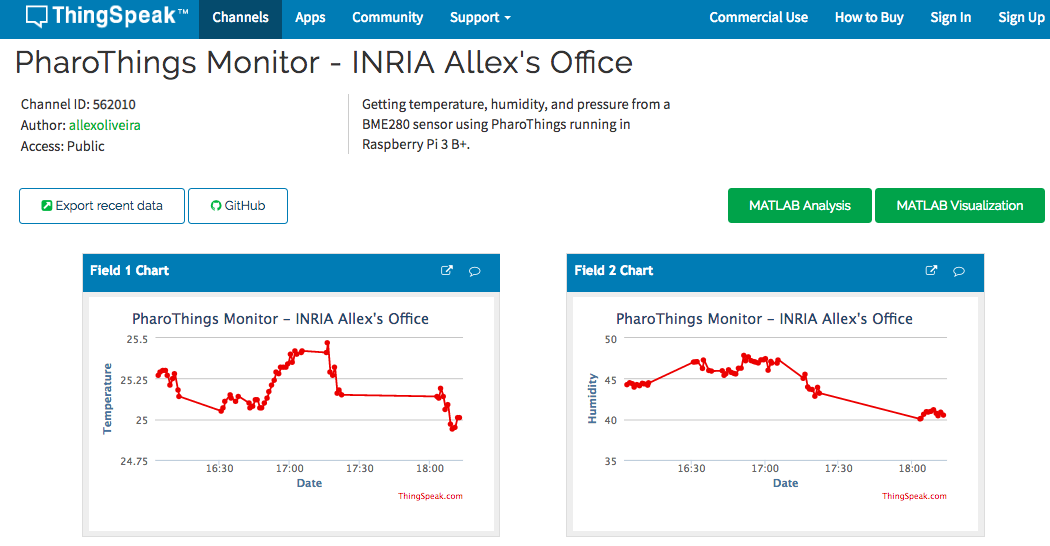
\includegraphics[width=0.85\textwidth]{/Users/allexoliveira/PharoThingsBook/Booklet-APharoThingTutorial/_result/pdf/Chapters/Chap12BuildingaMiniWeatherStation/figures/pharothings-thingspeak.png}\caption{ThingSpeak Channel.\label{ThingspeakChannel}}\end{center}
\end{figure}




% lulu requires an empty page at the end. That's why I'm using
% \backmatter here.
\backmatter

% Index would go here

\end{document}
